
\documentclass[english]{article}

\pdfoutput=1

\usepackage[T1]{fontenc}
\usepackage[latin9]{inputenc}
\usepackage{verbatim}
\usepackage{float}
\usepackage{amsthm}
\usepackage{amsmath}
\usepackage{amssymb}
\usepackage{graphicx}
%\usepackage{multirow}
\usepackage{color}
\usepackage{url}
\usepackage{caption}
\usepackage{subcaption}
\usepackage{mathtools} 

\newcommand{\TODO}[1]{{\color{red}{[#1]}}}

\makeatletter

%%%%%%%%%%%%%%%%%%%%%%%%%%%%%% Textclass specific LaTeX commands.
\numberwithin{equation}{section}
%\numberwithin{figure}{section}
\theoremstyle{plain}
\newtheorem{thm}{\protect\theoremname}[section]
\theoremstyle{definition}
\newtheorem{defn}[thm]{\protect\definitionname}
\theoremstyle{remark}
\newtheorem{claim}[thm]{\protect\claimname}
\theoremstyle{plain}
\newtheorem{lem}[thm]{\protect\lemmaname}

\newtheorem*{lem*}{Lemma}

\theoremstyle{remark}
\newtheorem{rem}[thm]{\protect\remarkname}
\theoremstyle{plain}
\newtheorem{corollary}[thm]{\protect\corollaryname}
\theoremstyle{plain}
\newtheorem{proposition}[thm]{\protect\propositionname}
%%%%%%%%%%%%%%%%%%%%%%%%%%%%%% User specified LaTeX commands.
%\usepackage{slashbox}

\usepackage{babel}
\providecommand{\claimname}{Claim}
\providecommand{\definitionname}{Definition}
\providecommand{\lemmaname}{Lemma}
\providecommand{\remarkname}{Remark}
\providecommand{\theoremname}{Theorem}
\providecommand{\corollaryname}{Corollary}
\providecommand{\propositionname}{Proposition}


\newcommand{\reals}{\mathbb{R}}
\newcommand{\RL}{\mathbb{R}^L}
\newcommand{\CL}{\mathbb{C}^L}
\newcommand{\RN}{\mathbb{R}^L}
\newcommand{\RNN}{\mathbb{R}^{N\times N}}
\newcommand{\CNN}{\mathbb{C}^{N\times N}}
\newcommand{\inner}[1]{\left\langle {#1} \right\rangle}
\newcommand{\hx}{\hat{x}} 

\newcommand{\SNR}{{\textsf{SNR}}} 

\begin{document}

\title{Estimation below the detection limit}


\author{Tamir Bendory}
\maketitle

\begin{abstract}
	Here comes the abstract
\end{abstract}

\section{Introduction}

In this paper, we consider the problem of estimating a set of signals $x_1,\ldots,x_K$ which appear multiple times in unknown, random, locations in a data sequence $y$. The data may also contain background information -- independent of the signals -- which is modeled as noise.
For one-dimensional signals, the data can be thought of as a long time series and the signals as repetitive short events. For two-dimensional signals, the data is a big image that contains many smaller images.  
The problem is then to estimate the signals $x_1,\ldots x_K$ from $y$. This
model appears, in different noise levels, in many applications, including spike sorting~\cite{lewicki1998review}, passive radar~\cite{gogineni2017passive} and system identification~\cite{ljung1998system}.
In Section~\ref{sec:model} we provide a precise mathematical formulation of the problem.

If the noise level is negligible, estimating the signals is easy.
One can detect the signal occurrences in the data sequence and then estimate the signals using clustering and averaging.
Even in higher noise level regimes, clever methods based on template matching, such as those used in structural biology~\cite{heimowitz2018apple} and radar~\cite{gogineni2017passive}, may work.
However, in the low signal--to--noise (\SNR) regime, detection of individual signal occurrences is impossible as clarified in Section~\ref{sec:model}. In Figure~\ref{fig:example} we demonstrate an instance of the problem in different noise levels. Figure~\ref{fig:data2D_clean} shows a excerpt of a big image that contains many repetitions of $21\times 21$ small image. The small image is a downsampled version of TKTK, which is shown in Figure~\ref{fig:signal2D_clean}. In Figures~\ref{fig:data2D_noisy_02} and~\ref{fig:data2D_noisy_1} the same excerpt is shown with the addition of i.i.d.\ Gaussian noise with standard deviations of $0.2$ and $1$, respectively.  

In this work we focus on the low $\SNR$ regime. To estimate the signal we use autocorrelation analysis of the data. 
In a nutshell,
the method consists of two stages. First, we estimate a mix of the low order autocorrelations of the signals from the data. These quantities can
be estimated to any desired accuracy if the signals appear enough times in the measurements, without the need to detect individual occurrences. Then, the signals are estimated from the mixed autocorrelations.
In Section~\ref{sec:autocorrelation}, we elaborate on our method  and show that if $K$ not too large, it is possible to estimate the signals, in any $\SNR$ level and to any desired accuracy.
This holds if each signals appears enough times in the data and the signals are sufficiently spaced. 
Interestingly, alternative methods which are often employed in similar estimation problems, such as expectation-maximization (EM) or Monte-Carlo Markov Chain (MCMC), seems to be intractable for this problem. In Figure~\ref{fig:signal2D_LS} we show an example for estimation of the signals where the data is contaminated with noise with standard deviation of $\sigma=1$ as presented in Figure~\ref{fig:data2D_noisy_1}. The normalized error between the signal and its estimation is TKTK. In Section~\ref{sec:numerics} we provide the details of this experiment and show additional experiments with $K>1$. 


\begin{figure}[ht!]
    \advance\leftskip-4cm
   \advance\rightskip-4cm

%	\centering

	\begin{subfigure}{.5\textwidth}
		\centering
	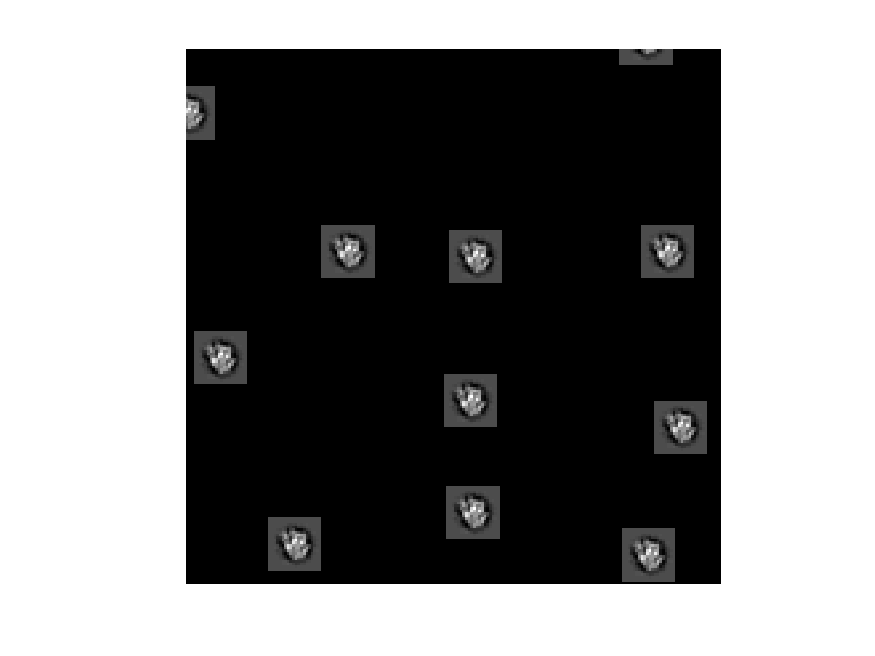
\includegraphics[scale=0.5]{data2D_clean}
\caption{Excerpt of clean data}
\label{fig:data2D_clean}
	\end{subfigure}%
	\begin{subfigure}{.5\textwidth}
	\centering
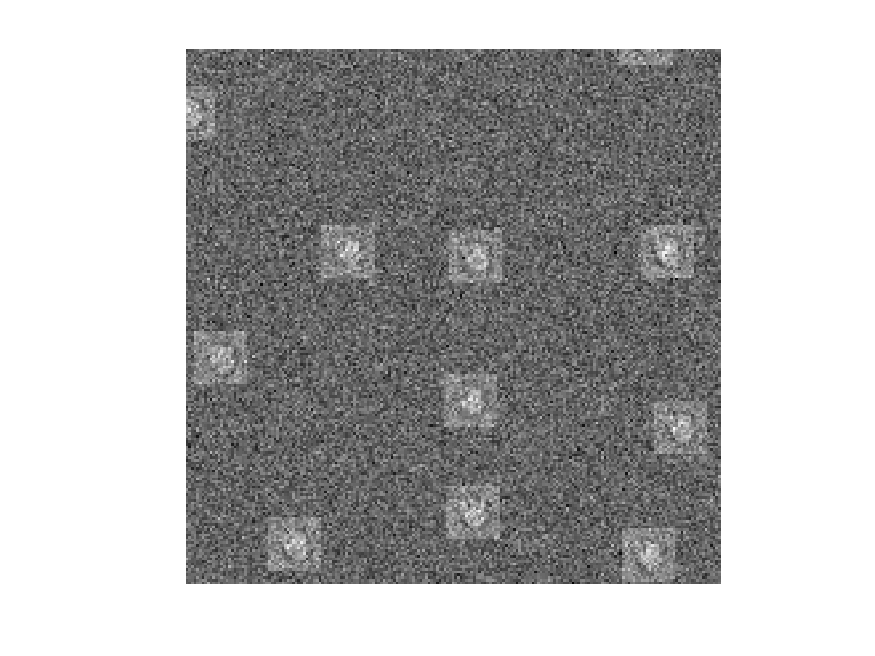
\includegraphics[scale=0.5]{data2D_noisy_02}
\caption{Excerpt of noisy data with $\sigma=0.2$}
\label{fig:data2D_noisy_02}
	\end{subfigure}
	\begin{subfigure}{.5\textwidth}
	\centering
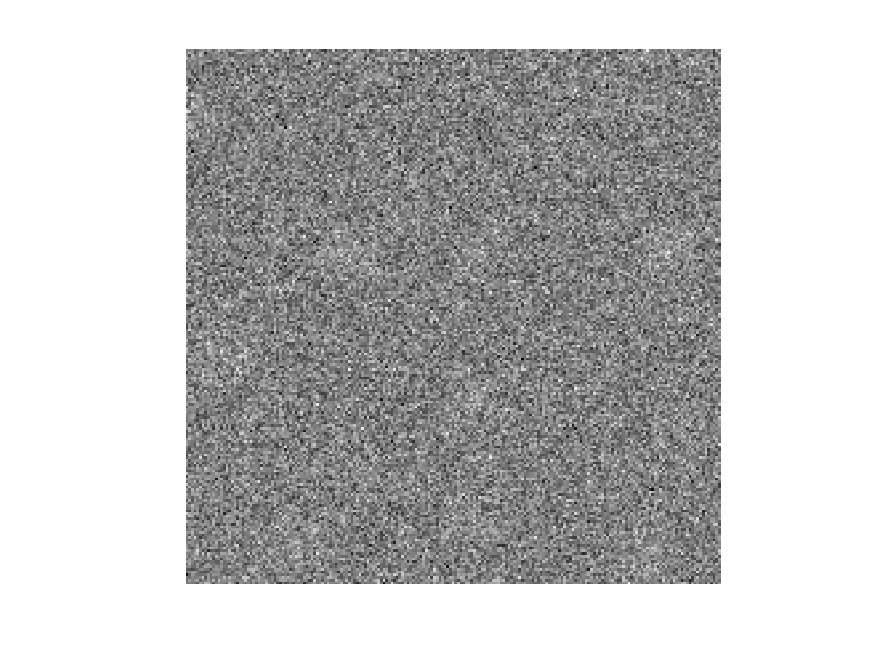
\includegraphics[scale=0.5]{data2D_noisy_1}
\caption{Excerpt of noisy data with $\sigma=1$}
\label{fig:data2D_noisy_1}
\end{subfigure}

	\begin{subfigure}{.5\textwidth}
	\centering
	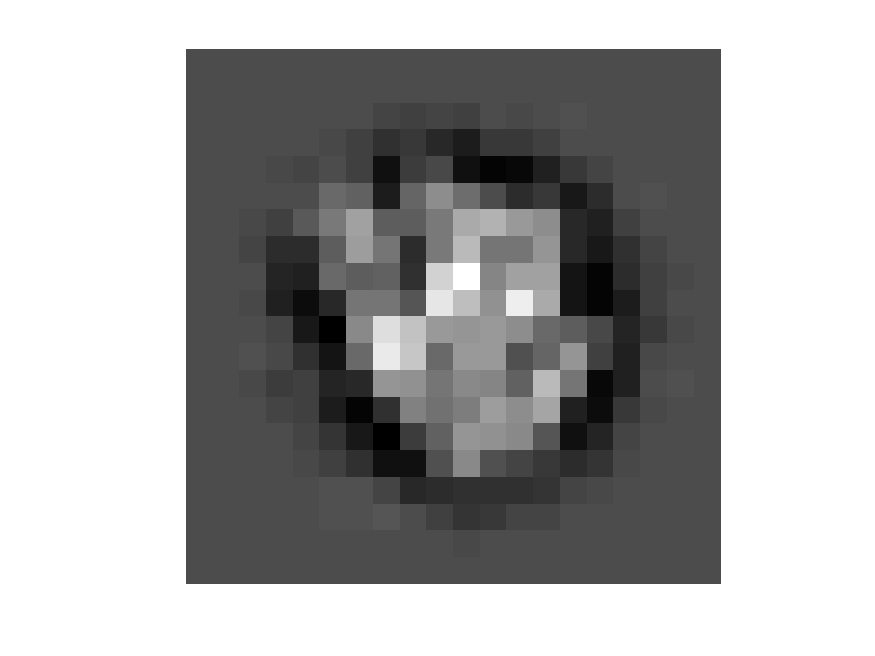
\includegraphics[scale=0.5]{signal2D_clean}
	\caption{Clean signal}
	\label{fig:signal2D_clean}
\end{subfigure}%
\begin{subfigure}{.5\textwidth}
	\centering
	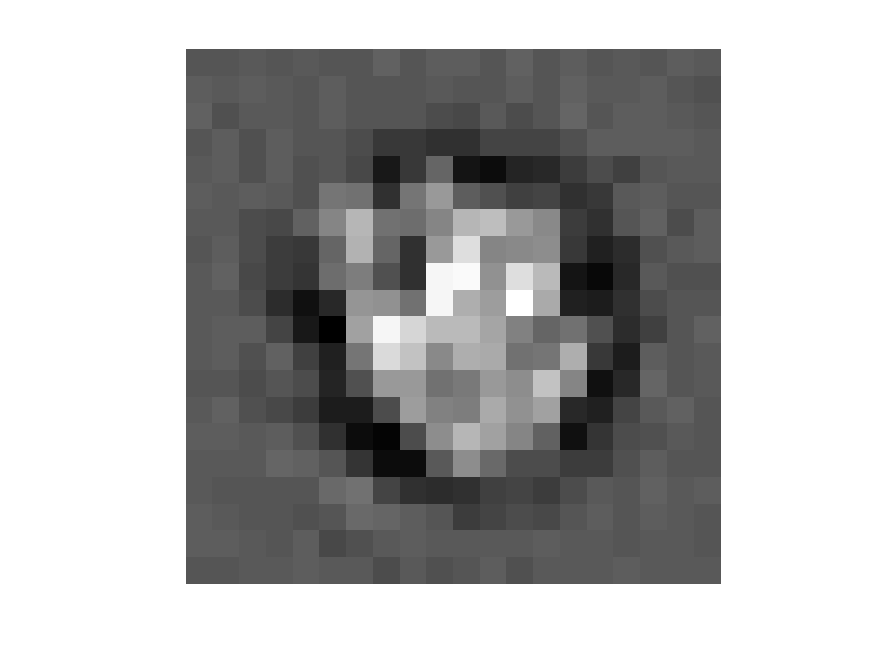
\includegraphics[scale=0.5]{signal2D_LS_all_images}
	\caption{710K micrographs, $M=561Mega$, error  = $0.05062$}
	\label{fig:signal2D_LS}
\end{subfigure}
\begin{subfigure}{.5\textwidth}
	\centering
	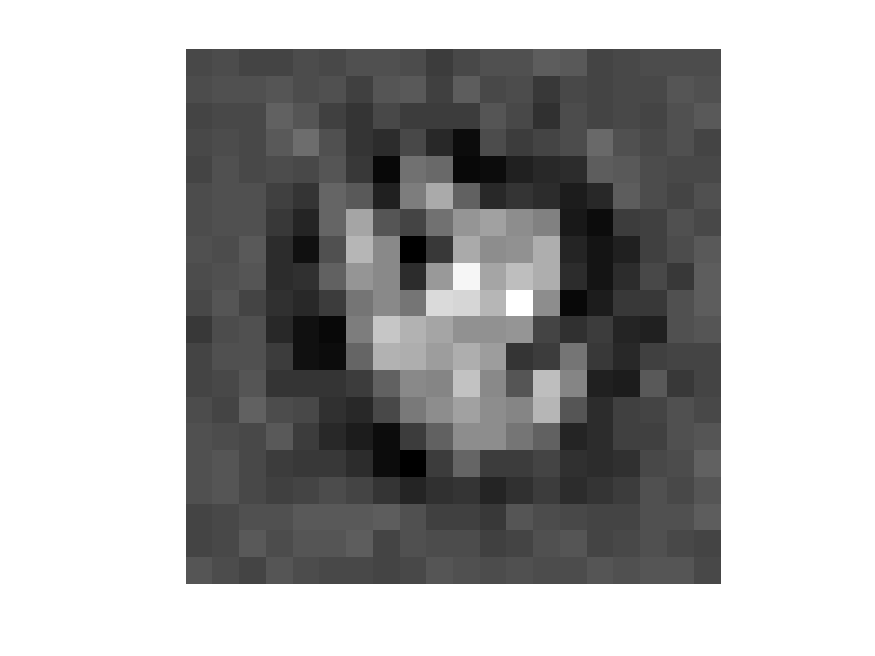
\includegraphics[scale=0.5]{signal2D_LS_exp1}
	\caption{Recovery with 140K micrographs and $M = 110Mega$, error = ? }
	\label{fig:signal2D_RRR}
\end{subfigure}

\caption{Example}
\label{fig:example}
\end{figure}



This work is primely motivated by  innovative technologies for single particle reconstruction, such as cryo-electron microscopy (cryo--EM) and X-ray Free--Electron Laser (XFEL). The acquired data in these modalities is contaminated with high noise levels. Therefore, any molecule reconstruction algorithm must take  the challenging $\SNR$ level into account.  In the last part of this manuscript, we will revisit the cryo--EM problem and draw connections with the estimation problem under consideration.


\section{Model}  \label{sec:model}

Let $x_1,\ldots,x_K\in\RL$ be the sought signals and let $y\in\RN$ be the data. For each $x_i$, we associate a binary signal  $s_i\in\{0,1\}^N$, referred to as the \emph{support signal} and let $s = \sum_{i=1}^Ks_i$. The non-zero values of $s_i$ indicates the locations of $x_i$ in $y$. If $s_i[n]=1$, then $y[n+j] = x_i[n+j]+\varepsilon[n+j]$ for $j=0,\ldots,L-1$.
We denote the cardinality of $s_i$ by $M_i$  and $M = \sum_{i=1}^{K}M_i$. We do not assume the knowledge of $M_i$'s, neither of $M$.


The support signals are generated by the following generative model. The signal $s$ is initialized with zeros.
First, an index $i_1$ is drawn uniformly from $\{1,\ldots,N\}$ and we set $s[i_1]=1$. A second index $i_2$ is then drawn uniformly from $\{1,\ldots,N\}$. If $\vert i_2-i_1\vert \geq L$,
then we set $s[i_2]=1$, otherwise we keep $s[i_2]=0$ and draw a new index  from uniform distribution. We then proceed adding  non-zero entries to $s$,  while keeping the separation condition until some halting criterion is obtained. Ultimately, each  non-zero value of $s$ is associated with one of the $s_i$'s uniformly over  $\{1,\ldots,K\}$. We note that if the support is sparse enough, this generative model can be approximated by a simple Bernoulli process which takes the values of one and zero with probabilities  $M/N$ and $1-M/N$, respectively.

The simplest way to present the forward model is a mix of blind deconvolution problems between the support signals and the unknown signals
\begin{equation}
y = \sum_{i=1}^K x_i\ast s_i + \varepsilon,\quad \varepsilon\sim\mathcal{N}(0,\sigma^2 I).
\end{equation}
We model the background information as i.i.d.\ Gaussian noise with zero mean and $\sigma^2$ variance. 
The goal is to estimate $x_1,\ldots,x_K$ from $y$.

Blind deconvolution is a longstanding problem, arising in a variety of engineering and scientific applications, such as astronomy, communication, image deblurring, system identification and optics; see~\cite{jefferies1993restoration,shalvi1990new,ayers1988iterative,abed1997blind}, just to name a few. Clearly, without additional information on the signal, blind deconvolution is ill-posed. In our case, the prior information is that $s$ is a binary, sparse, signal. 
Other settings of blind deconvolution problems have been analyzed recently under different settings, see for instance~\cite{ahmed2014blind,li2016identifiability,li2016rapid,ling2015self,ling2017blind,chi2016guaranteed}
where the focus is on high $\SNR$ regimes.



In our setup, the support signals $s_1,\ldots,s_K$ are the \emph{latent} variables of the problem. Indeed, in many blind deconvolution applications the goal is merely to estimate one of the unknown signals. For instance, in image deblurring, both the blurring
kernel and the high-resolution image are unknown, but the prime goal is only
to sharpen the image.
If $x$ is known and $K=1$, then  $s$ can be estimated by linear programming  in the high $\SNR$ regime~\cite{de2012exact,duval2015exact,bendory2016robust,bendory2017robust,bernstein2017deconvolution}. However, in the low $\SNR$ regime, estimating $s$ is impossible. To see that, suppose that an oracle provides us $M$ windows of length $W>L$, each contain one occurrence of $x$. Put it differently, we get a series of windows, each one contains a signal at unknown location.
Estimating the first entry of the signals within each  window is an essentially easier problem the detecting the support of $s$ since the windows are given to us by the oracle. Apparently, this problem, called alignment or synchronization, is impossible in the low $\SNR$ regime.
For instance, the variance of any estimator is, at best, proportional to $\sigma^2$ and independent of the number of windows, even if $x$ is known~\cite{aguerrebere2016fundamental}. Therefore, we conclude that that detecting the non-zero values of $s$ is impossible in low \SNR. 

In the next section we show that if $M$ is large enough, then estimating the signals is possible, in any $\SNR$ level and to any accuracy, although we cannot detect their occurrences in $y$. 



\section{Autocorrelation analysis}   \label{sec:autocorrelation}

Our method for estimating the signals relies on two pillars. 
First, we use the autocorrelation functions of the data to estimate a mix (i.e., linear combination) of the $K$ signals autocorrelations. The mixed autocorrelation can be estimated to any accuracy, in any $\SNR$ level, if $M$ is large enough and the separation condition on the support is held. Then, we use least-squares (LS) estimator to estimate the signals from their mixed autocorrelation. From pedagogical reasons, we start with the second stage of recovering signals from their autocorrelations. In this section we mainly discuss the uniqueness of the mapping from the autocorrelation to the signals. Concrete algorithms will be discussed in the next section.

For the purpose of this paper, we need the first three (aperiodic) autocorrelation functions of a signal $z\in\mathbb{R}^W$, defined as
\begin{align} \label{eq:autocorrelations}
a_z^1 &= \sum_{i=0}^{W-1} z[i], \nonumber\\
a_z^2[\ell] &= \sum_{i=0}^{W-1-\ell} z[i]z[i+\ell], \nonumber\\
a_z^3[\ell_1,\ell_2] &= \sum_{i=0}^{W-1-\max\{\ell_1,\ell_2\}} z[i]z[i+\ell_1]z[i+\ell_2]. 
\end{align}
Note that the autocorrelation functions are symmetric so that $a_z^2[\ell] = a_z^2[-\ell]$ and $a_z^3[\ell_1,\ell_2] = a_z^3[-\ell_1,-\ell_2]$. 

A one-dimensional signal is determined uniquely by its third-order auto-correlation:
\begin{proposition}
	Suppose that $z[0]$ and $z[L-1]$ are non-zeros. Then, a signal $z\in\mathbb{R}^W$ is determined uniquely from  $a_z^2$ and $a_z^3$.
	\begin{proof}
		From the second-order autocorrelation, we ge
		\begin{equation*}
		a_z^2[L-1] = z[0]z[L-1]\neq 0.
		\end{equation*}
		Then, from the third-order autocorrelation we can compute $z[k]$ for all $k=0,\ldots L-1$ by
		\begin{eqnarray}
		a_z^3[k,L-1] = z[0]z[k]z[L-1].
		\end{eqnarray}
	\end{proof}
\end{proposition}
We note that the length of the signal can be easily derived from the second-order autocorrelation of the signal. Therefore, the assumption that $z[0]$ and $z[L-1]$ is met in practice. We also note that for one-dimensional signals, the second-order autocorrelation does not determined the signals uniquely~\cite{beinert2015ambiguities,bendory2017fourier}. This is not the case for dimensions greater than one, in which almost all signals are determined uniquely from their aperiodic autocorrelations, up to sign (phase in the complex case) and reflection through the origin (with conjugation in the complex case)~\cite{hayes1982reconstruction,hayes1982reducible,bendory2017fourier}. The sign ambiguity can be resolved by the mean of the signal if it is not zero. However,  in order to determine the reflection symmetry ($Z_2$ symmetry), one needs to use the third moment.

The heterogeneous case $K>1$ was explored for periodic autocorrelation functions. The aperiodic autocorrelations are the periodic autocorrelations of signals padded by zeros. Therefore, the following results hold for our setup as well  \TODO{we should be prudent here to make sure that this set does not ``fall'' in the zero measure}. In~\cite{bandeira2017estimation}, it was shown that a mix of $K$ third-order autocorrelations determine  a finite list of $K$ generic signals when 
\begin{itemize}
	\item $K=2$ when $L>1$,
	\item $K=3$ when $L>12$,
	\item $K=4$ when $L>18$,
	\item $5\leq K\leq 15$ when $L\geq 6K-5$.	
\end{itemize}
The authors conjecture that for $K>15$, $L\geq 6K-5$ is enough. Recently, Joe told use that he has proven that there is unique mapping in the same regime.  
This also holds for arbitrary weights $\gamma_i$ which are rational fractions.

\TODO{Where we should refer to Gianakis's paper?}

We are moving forward to discuss the second question of how to estimate the autocorrelation of the signals from the data. 
The analysis is conducted in the asymptomatic regime where $M_1,\ldots,M_K,N\to\infty$. We define the ratios 
\begin{equation}
\gamma_i = \frac{M_i L}{N},
\end{equation}
and $\gamma = \sum_{i=1}^K\gamma_i$.
Under the separation condition, we have $\gamma\leq\frac{L}{2L-1}\approx 1/2$.
The main insight is that if $s$ satisfies the separation condition, then the first $L$ entries of the data autocorrelations converge to a $\gamma$ scaled version of a mix of the signals autocorrelations:
\begin{align}
\lim_{N\to\infty} a_y^1 &= \sum_{i=1}^K\gamma_i a_{x_i}^1, \\
\lim_{N\to\infty} a_y^2[\ell] &= \sum_{i=1}^K\gamma_i a_{x_i}^2[\ell] +\sigma^2\delta[\ell],\\
\lim_{N\to\infty} a_y^3[\ell_1,\ell_2] &= \sum_{i=1}^K\gamma_i a_{x_i}^3[\ell_1,\ell_2] + \sigma^2\left(\sum_{i=1}^K\gamma_i a_{x_i}^1\right)(\delta[\ell_1,0]+\delta[0,\ell_2]+\delta[\ell_1,\ell_2]),
\end{align}
for $\ell,\ell_1,\ell_2=0,\ldots L-1$.
These relations are proved in Appendix~\ref{sec:autocorrelation_computation}. The analysis is similar to~\cite{bendory2017bispectrum,boumal2017heterogeneous}, yet a special caution should be taken with the noise dependencies. This means that given $M_1,\ldots,M_K$ and $\sigma^2$ and $K$ does not exceed the limit for uniqueness, the one can estimate the signals from the third-order autocorrelation of the data. In other words, the signals can be estimated in asymptotic estimation rate of $\sigma^6/N$.


If the noise level $\sigma^2$ is known, then for $K=1$, one can estimate $M$ from only the first two moments, namely, with estimation rate of $\sigma^4/N$.
\begin{proposition}
	Let $K=1$. Then, 
	\begin{equation*}
	\frac{M}{N} = \frac{(a^1_y)^2}{\sum_{j=0}^{L-1}a_y^2[j]-\sigma^2}.
	\end{equation*}
	\begin{proof}
The relation is proved by plugging the definitions of the signal autocorrelations into the right-hand side of the equation~\eqref{eq:autocorrelations}. 	
\end{proof}
\end{proposition}

If we assume that $s$ is sparse, then by ignoring the separation condition, one can describe the generative process of $s$ as a Bernoulli process with parameter $M/N$. Therefore, in low \SNR  one can estimate the parameter that control this statistical process, although cannot estimate individual entries.

Estimating $\sigma$ and $M$? 


\section{Numerical experiments}   \label{sec:numerics}



\section{Conclusion} 
Here we conclude the paper: cryo -- EM, structured background, without separation, heterogeneity
In particular, in cryo--EM, multiple projections of a molecule (signal), taken
from unknown viewing directions, are recorded on two-dimensional detector
array. Current algorithms try to detect these projections in a low SNR regime
and then use them for the reconstruction process. Since the
Then, the reconstruction problem is to detect these projection, and then use
them to estimat
The data acquired in both technologies is composed of multiple projections
of a molecule (the signal), taken from unknown viewing direction, and drawn in
high noise level. The reconstitution problem is then to estimate the molecule
from this data.


\bibliographystyle{plain}
\bibliography{ref}



\appendix

\section{Autocorrelation estimations} \label{sec:autocorrelation_computation}
 
To analyze the asymptotic behavior of the data autocorrelation functions, we consider one signal $K=1$. The extension to $K>1$ is straightforward by averaging the contributions of all signal with the appropriates weights, see~\cite{boumal2017heterogeneous}. 

Let us define
\begin{equation}
\gamma = \lim_{N\to\infty} \frac{M_NL}{N}<1.
\end{equation}
By assuming $M_N=\Omega(N)$, we also have $\gamma>0$.
We start by considering the first autocorrelation of the data
\begin{equation}
a_y^1 = \sum_{i=0}^{N-1} y[i] = \frac{1}{N/L}\sum_{j=0}^{M_N-1}\frac{1}{L}\sum_{i=0}^{L-1}x[i] + \underbrace{\frac{1}{N}\sum_{i=0}^{N-1}\varepsilon[i]}_{\text{noise term}} \xrightarrow{a.s.}\gamma a_x^1,
\end{equation}
where the noise term converges to zero almost surely (a.s.) by the law of large numbers.

We proceed with the second moment for fixed $\ell\in[0,\ldots,L-1]$. Then, we can compute, 
\begin{equation}
\begin{split}
a_y^2[\ell] & = \frac{1}{N}\sum_{i=0}^{N-1-\ell}y[i]y[i+\ell] \\
& \underbrace{\frac{1}{N}\sum_{j=1}^{M_N}\sum_{i=0}^{L-\ell-1}x[i]x[i+\ell]}_{\text{signal term}} + \underbrace{\frac{1}{N}\sum_{i=0}^{N-1}\varepsilon[i]\varepsilon[i+\ell]}_{\text{noise term}},
\end{split}
\end{equation}
where the cross terms between the signal and the noise almost surely vanish in the limit. 

We treat the signal and noise terms separately. We first break the signal term into $M_N$ different sums, each contains one copy of the signal, and get
\begin{equation} \label{eq:2nd_moment_signal_term}
\frac{1}{N}\sum_{j=1}^{M_N}\sum_{i=0}^{L-\ell-1}x[i]x[i+\ell] = \frac{M_NL}{N}\frac{1}{L}\sum_{i=0}^{L-\ell-1}x[i]x[i+\ell] = \gamma a_x^2[\ell].
\end{equation}
Similarly, for $\ell\neq 0$, we can break the noise term into a sum of independent terms 
\begin{equation}
\frac{1}{N}\sum_{i=0}^{N-1-\ell} \varepsilon[i]\varepsilon[i+\ell] = \frac{1}{\ell}\sum_{i=0}^{\ell-1}\frac{1}{N/\ell}\sum_{j=0}^{N/\ell -1} \varepsilon[j\ell + i] \varepsilon[(j+1)\ell + i].
\end{equation}
Each term of $\frac{1}{N/\ell}\sum_{j=0}^{N/\ell -1} \varepsilon[j\ell + i] \varepsilon[(j+1)\ell + i]$ is an average of $N/\ell$ independent terms with expectation zero, and therefore converge to zero almost surely as $N\to\infty$.
If $\ell=0$, 
\begin{equation}
\frac{1}{N}\sum_{i=0}^{N-1} \varepsilon[i]^2 \xrightarrow{a.s.} \sigma^2.
\end{equation}

We are now moving to the third-order autocorrelation. Let us fix $\ell_1\geq\ell_2$ and recall that 
\begin{equation*}
a_y^3[\ell_1,\ell_2] = \sum_{i=0}^{N-1-\ell_1} y[i]y[i+\ell_1]y[i+\ell_2]. 
\end{equation*}
Writing explicitly in terms of signal and noise, this sum can be broken into eight partial sums. The first contains only signal terms and converges to $\gamma a_x^3$ from the same reasons as~\eqref{eq:2nd_moment_signal_term}. Three other partial sums contain the product of two signal entries and one noise term. Since the noise is independent of the signal, then these terms go to zero almost surely.

We next analyze the contribution of triple product of noise terms. For $\ell_1\neq 0$, this sum can be formulate as follows:
\begin{equation*}
\sum_{i=0}^{N-1-\ell_1} \varepsilon[i]\varepsilon[i+\ell_1]\varepsilon[i+\ell_2] = \frac{1}{\ell_1}\sum_{i=0}^{\ell_1-1}\frac{1}{N/\ell_1}\sum_{j=0}^{N/\ell_1 -1 }\varepsilon[j\ell_1+i]\varepsilon[(j+1)\ell_1+i]\varepsilon[j\ell_1+i+\ell_2].
\end{equation*}
For each fixed $i$, we sum of over $N/\ell_1$ independent variables that goes to zero almost surely. For $\ell_1=\ell_2=0$, we get a some of $N$ independent variables, each is a triple product of Gaussian variables with zero mean. Therefore, it is also converges to zero. 

To complete the analysis, we consider the three terms composed of the product of two noise terms and one signal entry. Most of these terms converges to zero almost surely because of interdependency between the noise entries. For $\ell_1=0, \ell_2=0$ and $\ell_1=\ell_2$,  a simple computation shows that the sum converges to $\gamma\sigma^2a_x^1$.


\end{document}

